\documentclass{article}
\usepackage[utf8]{inputenc}
\usepackage{amsmath}
\usepackage{amsfonts}
\usepackage{graphicx}

\title{Discussion Assignment Unit 6\\
Math 1201 - College Algebra.
}
\author{Jasper Albert Nri}
\date{October 2021}


\begin{document}

\maketitle


\section*{PART 1}
\title\textbf{QUESTION}\\
First, create 3 equations of the form ${ax +by +cz=d}$, where a, b, c, and d are constants (integers between -5 and 5). For example, ${x+2y-z=-1}$. Perform on your system to obtain a row-echelon form and the solution.\\
Go to the 3D calculator website GeoGebra: www.geogebra.org/3d?lang=pt and enter each of the equations.\\
\\\title\textbf{SOLUTION}
The equations i will be using are
$${x-y+z=4}$$
$${3x-2y-z=-2}$$
$${4x+3y-2z=5}$$
Writing the augmented matrix
$$
\begin{bmatrix}
1 & -1 &  1 & | &  4\\
3 &  2 & -1 & | & -2\\
4 & -3 & -2 & | &  5\\
\end{bmatrix}
$$
Performing row operations to obtain row-echelon form.
$${
    -3R_{1}+R_{2}=R_{2}\rightarrow\begin{bmatrix}
        1 & -1 &  1 & | &   4\\
        0 &  5 & -3 & | & -14\\
        4 & -3 & -2 & | &   5\\
    \end{bmatrix}
}$$
$${
    -4R_{1}+R_{3}=R_{3}\rightarrow\begin{bmatrix}
        1 & -1 &  1 & | &   4\\
        0 &  5 & -3 & | & -14\\
        0 &  1 & -6 & | & -36\\
    \end{bmatrix}
}$$

$${
    \text{Interchange }R_{2}\text{ and }R_{3} \rightarrow\begin{bmatrix}
        1 & -1 &  1 & | &   4\\
        0 &  1 & -6 & | & -36\\
        0 &  5 & -3 & | & -14\\
    \end{bmatrix}
}$$
Then, 
$${
    -5R_{2}+R_{3}=R_{3}\rightarrow
    \begin{bmatrix}
        1 & -1 &  1 & | &   4\\
        0 &  1 & -6 & | & -36\\
        0 &  0 & 27 & | & 166\\
    \end{bmatrix}
}$$
$${
    \frac{1}{27}R_{3}=R_{3}\rightarrow
    \begin{bmatrix}
        1 & -1 &  1 & | &   4\\
        0 &  1 & -6 & | & -36\\
        0 &  0 &  1 & | & \frac{166}{27}\\
    \end{bmatrix}
}$$

$${ x - y + z = 4}$$
$${y-6z=-36}$$
$${z=\frac{166}{27}}$$
Substituting z into ${y-6z=-36}$
$${y=-36+6z}$$
$${y=-36+6\left(\frac{166}{27}\right)}$$
$${y=\frac{996}{27}-36}$$
$${y=\frac{24}{27}}$$

Substituting z and y into ${x-y+z=4}$
$${x-y+z=4}$$
$${x=4+y-z}$$
$${x= 4 + \frac{24}{27} - \frac{166}{27}}$$
$${x=\frac{108+24-166}{27}}$$
$${x=\frac{132-166}{27}}$$
$${x=-\frac{34}{27}}$$
So, the solution is $${\left( -\frac{34}{27},\frac{24}{27},\frac{166}{27} \right)}$$
These are the points of intersection between the three planes(Abramson, 2017).
The 3D graph of the equation is given below.\\
\\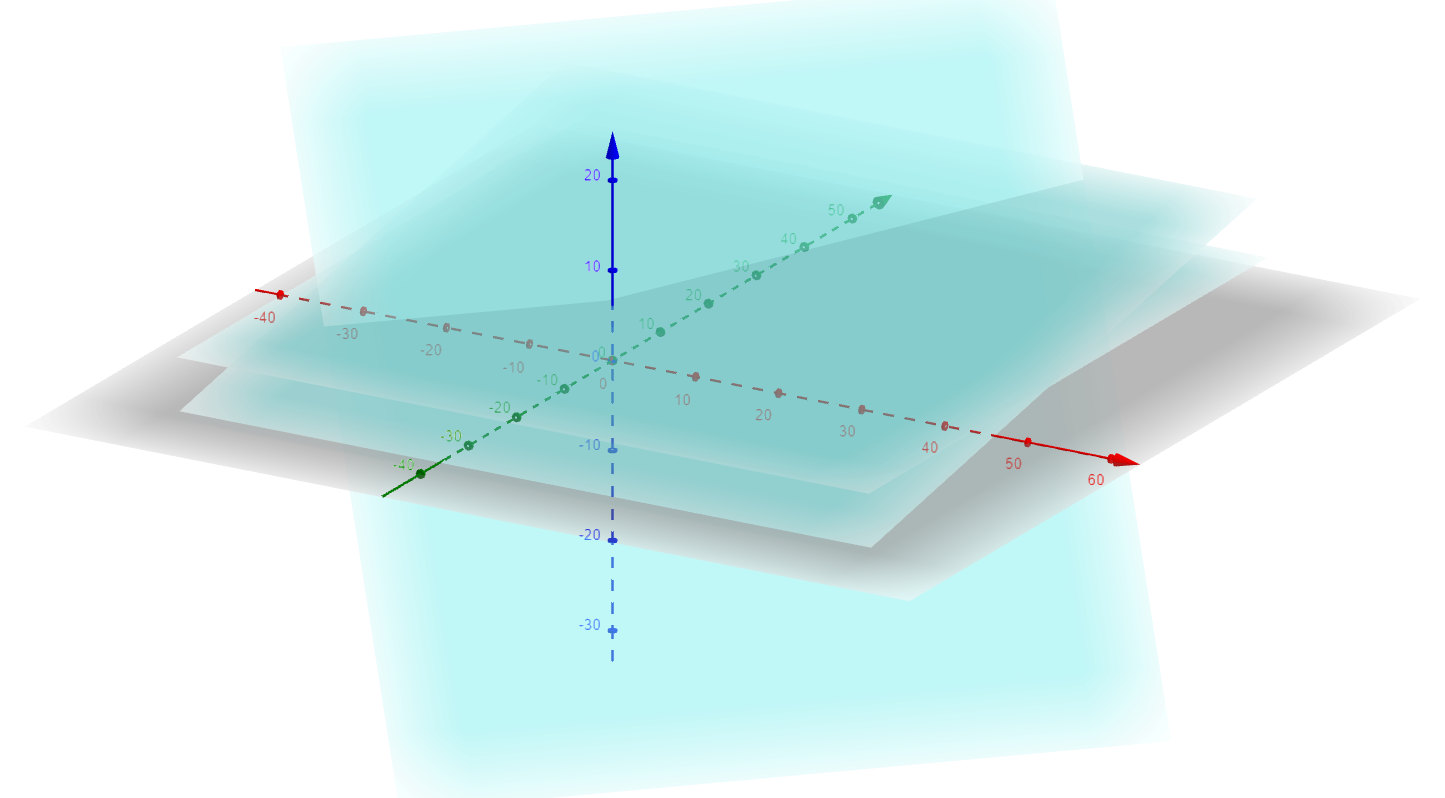
\includegraphics[scale = 0.25]{geo2}\\
$${}$$

\section*{PART 2}
\title\textbf{QUESTION}\\
After you have completed the first task, choose \textbf{ONE} of the following to complete your discussion post.\\
\textbf{4.} Give an example with 2 equations as simple as possible with 3 variables (at least 1 being non-linear, keeping z to the one power on both equations) and describe the potential of GeoGebra to study nonlinear systems.\\
\\\title\textbf{SOLUTION}
The First example of a non-linear system with a quadratic equation\\
$${3x^2+3y+z=10}$$
The 3D graph of the equation is given below.\\
\\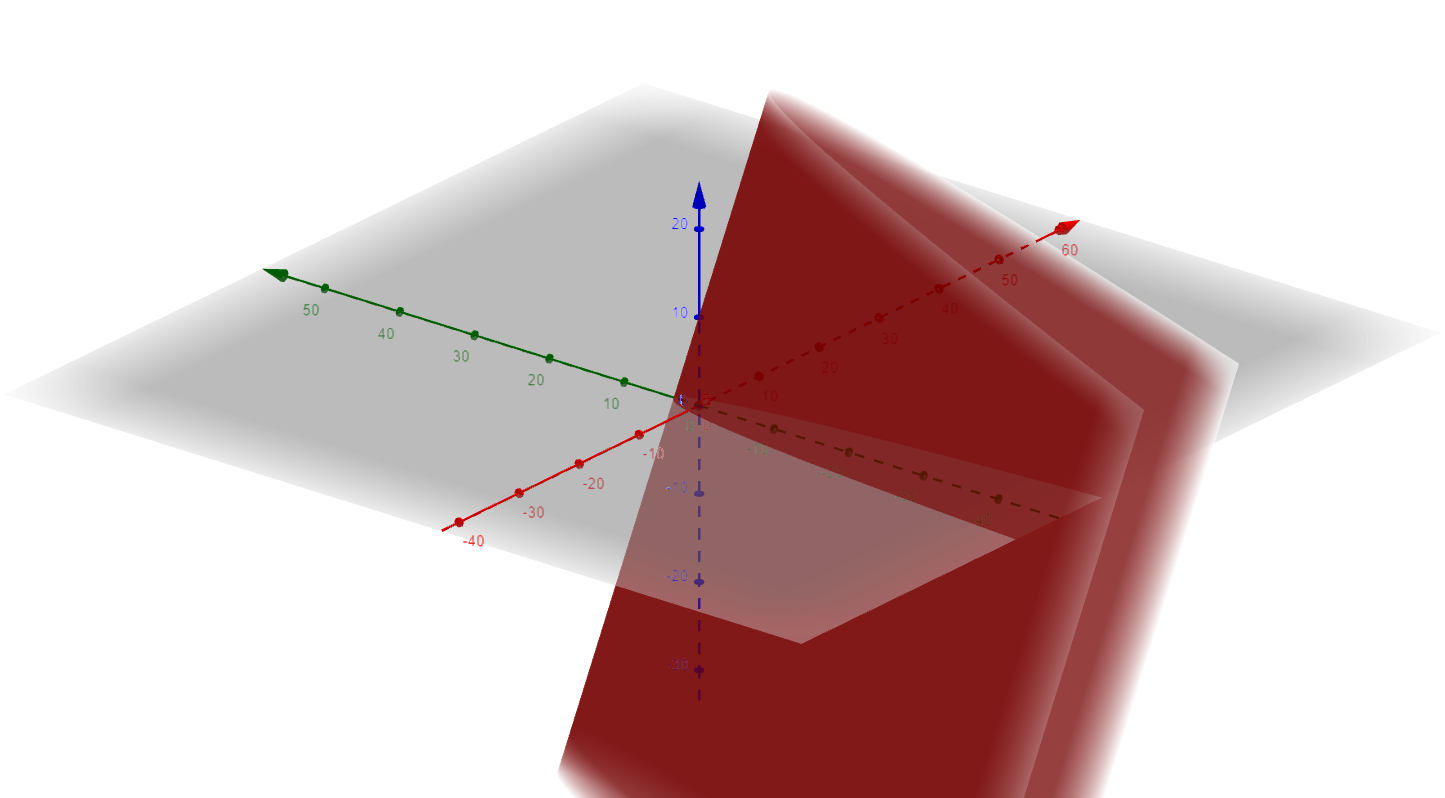
\includegraphics[scale = 0.25]{geo3}\\
The Second example of a non-linear system with a cubic equation\\
$${2x^2+4y^2+z=8}$$
The 3D graph of the equation is given below.\\
\\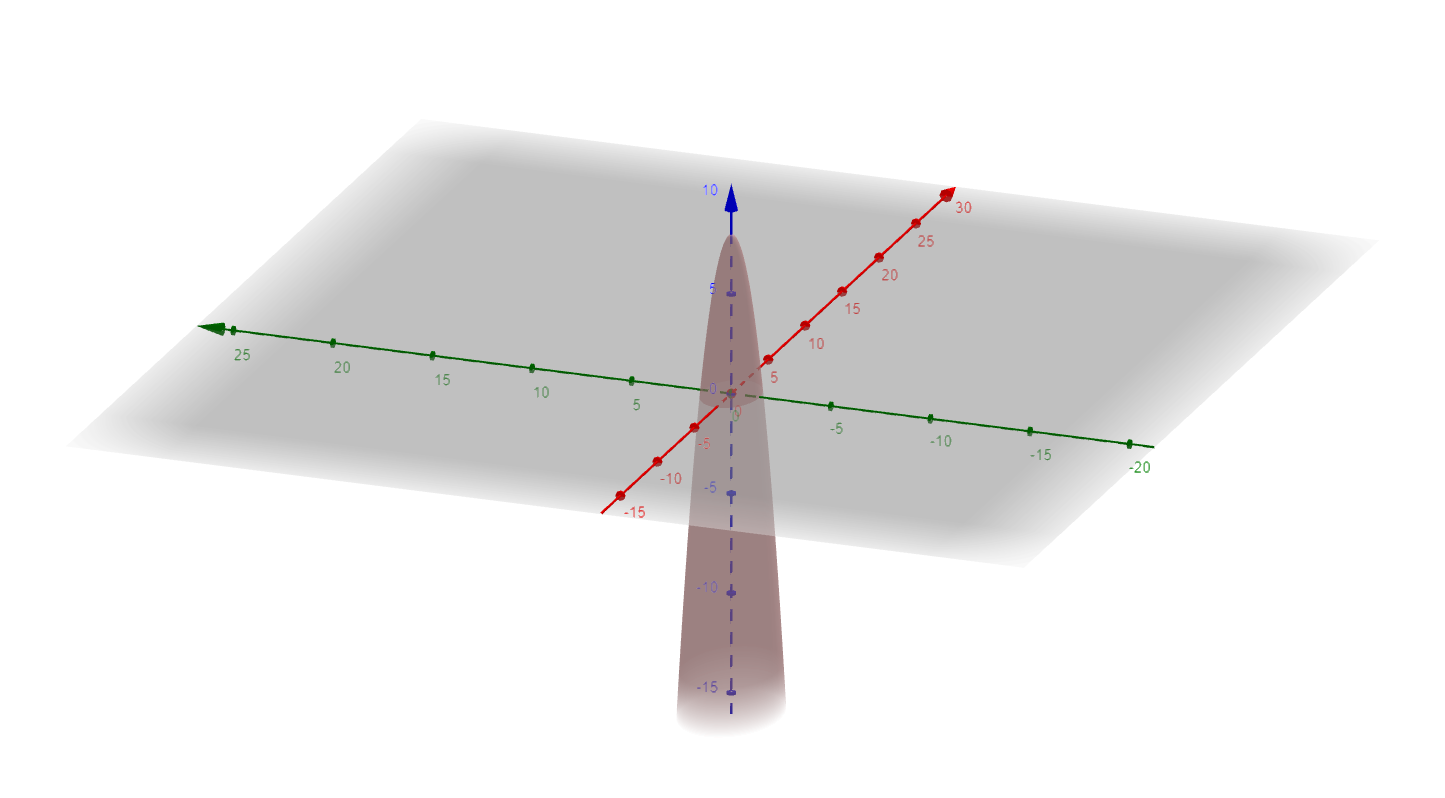
\includegraphics[scale = 0.25]{geo4}\\

Geogebra is a very useful tool plotting the graph of these equations for better visualisation of the points of intersection as it renders it in 3D.
\section*{References}
Abramson, J. (2017). \textit{Algebra and trigonometry}. OpenStax, TX: Rice University. Retrieved
from https://openstax.org/details/books/algebra-and-trigonometry
\end{document}